\documentclass[10.5pt]{article}

% ACL style package
\usepackage{acl}

% Standard packages
\usepackage{times}
\usepackage{latexsym}
\usepackage[T1]{fontenc}
\usepackage[utf8]{inputenc}
\usepackage{graphicx}
\usepackage{amsmath}
\usepackage{booktabs}
\usepackage{siunitx}
\usepackage{tabularx}
\usepackage{multirow}
\usepackage{ragged2e}

\title{The Role of Data Variety: Observing Cross-Skill Impacts Through Targeted LLM Unlearning}
\author{William Chastek \\ Joseph V. \\ John Phan \\
Team Name: NoobLP}

\begin{document}
\maketitle

\begin{abstract}
Large Language Models (LLMs) excel in multi-task reasoning, but their ability to selectively "unlearn" specific skills without degrading unrelated capabilities remains poorly understood. This study investigates the cross-domain impacts of unlearning mathematical reasoning in the DeepSeek-R1-Distill-Queen-1.5B model, employing two unlearning strategies: (1) fine-tuning on corrupted datasets and (2) gradient ascent. Both methods were found to cause unlearning with a combined average of 12.7\% decrease in the LLM's accuracy on math-related questions, and limited impact on other skill domains. With the highest impact being in the intruction following category wiht a 5\% average decrease in accruacy. Other categories were also affected, but the impact was marginal with a decrease in accuracy about 1\%.
\end{abstract}

\section{Introduction}
LLM unlearning has been a topic of interest since the development of very large LLM platforms such as ChatGPT, as a way to remove unwanted behaviors. In this context, “unlearning” pertains to modifying the model weights to forget a concept or skill. Currently, researchers used a combination of reinforcement learning\cite{mu2024rule}, as well as gradient ascent\cite{neel2020descenttodeletegradientbasedmethodsmachine} to unlearn unwanted behaviors or knowledge. Many reinforcement learning techniques require human input, which makes it hard to scale and gradient ascent approaches have shown to cause degradation in LLM performance outside of the unwanted behavior or knowledge. 

\section{Motivation}
Unlearning techniques are critical for adapting LLMs to evolving ethical and practical standards. However, unintended skill degradation poses risks—for instance, unlearning math might impair logical reasoning or data analysis. This work addresses two questions:
\begin{enumerate}
    \item How does unlearning a specific skill affect performance in related domains?
    \item Can unlearning methods be refined to minimize collateral damage?
\end{enumerate}

\section{Approach}
There are two phases to the project:

\subsection{Training}
The unlearning process was conducted in two different ways:
\begin{enumerate}
    \item \textbf{Corrupted Dataset:} Fine-tune the model on a corrupted or scrambled dataset.
    \item \textbf{Gradient Ascent:} Fine-tune the model on the original math dataset using gradient ascent to push the model away from correct math answers.
\end{enumerate}
\\
The corrupted dataset has three variants:
\begin{enumerate}
    \item \textbf{scrambled:} Answers are swapped across items so none remain correct.
    \item \textbf{val-modified:} Non-question numbers are modified but retain original digit lengths.
    \item \textbf{length-val-modified:} Non-question numbers are modified and digit lengths may change.
\end{enumerate}

Gradient ascent has two variants:
\begin{enumerate}
    \item \textbf{gradient-ascent:} Use the negative loss for ascent.
    \item \textbf{reduced-eos-gradient-ascent:} Same as gradient-ascent but reduce EOS token priority to discourage early stopping.
\end{enumerate}
\subsection{Testing}
We used the LiveBench LLM benchmark~\cite{livebench}, which covers six categories, and the Math500 dataset~\cite{lightman2023lets} to evaluate cross-domain effects. Two prompt templates were used:
\begin{enumerate}
    \item \textbf{Chain-of-Thought Prompting:}
    \begin{verbatim}
Please reason step by step, and put your 
final answer within \boxed{}.
{problem_text}
    \end{verbatim}
    \item \textbf{Direct Prompting:}
    \begin{verbatim}
{problem_text}. Place your final answer 
in a box with \boxed{}
    \end{verbatim}
\end{enumerate}
\section{Datasets and Models}
\subsection{Models}
The model used for experimentation was DeepSeek-R1-Distill-Qwen-1.5B from HuggingFace.
\subsection{Datasets}
The dataset used for fine-tuning the model was MATH\_algebra\_crowdsourced from the allenai/lila dataset\cite{Mishra2022Lila}, which can be found on HuggingFace. 
\\
For testing the dataset used was the Math500 dataset which is a subset of the prm dataset~\cite{lightman2023lets} using by OpenAi.


\section{Experiments and Results}
To see if the unlearning was successful, the original non-corrupted dataset was used for evaluation. Using the two prompt templates, Chain-of-Though(CoT) and direct prompting, for evaluation, the accuracy for each model was recorded in Figure 1 and Figure 2. 
\\
\begin{figure}[h]
    \centering
    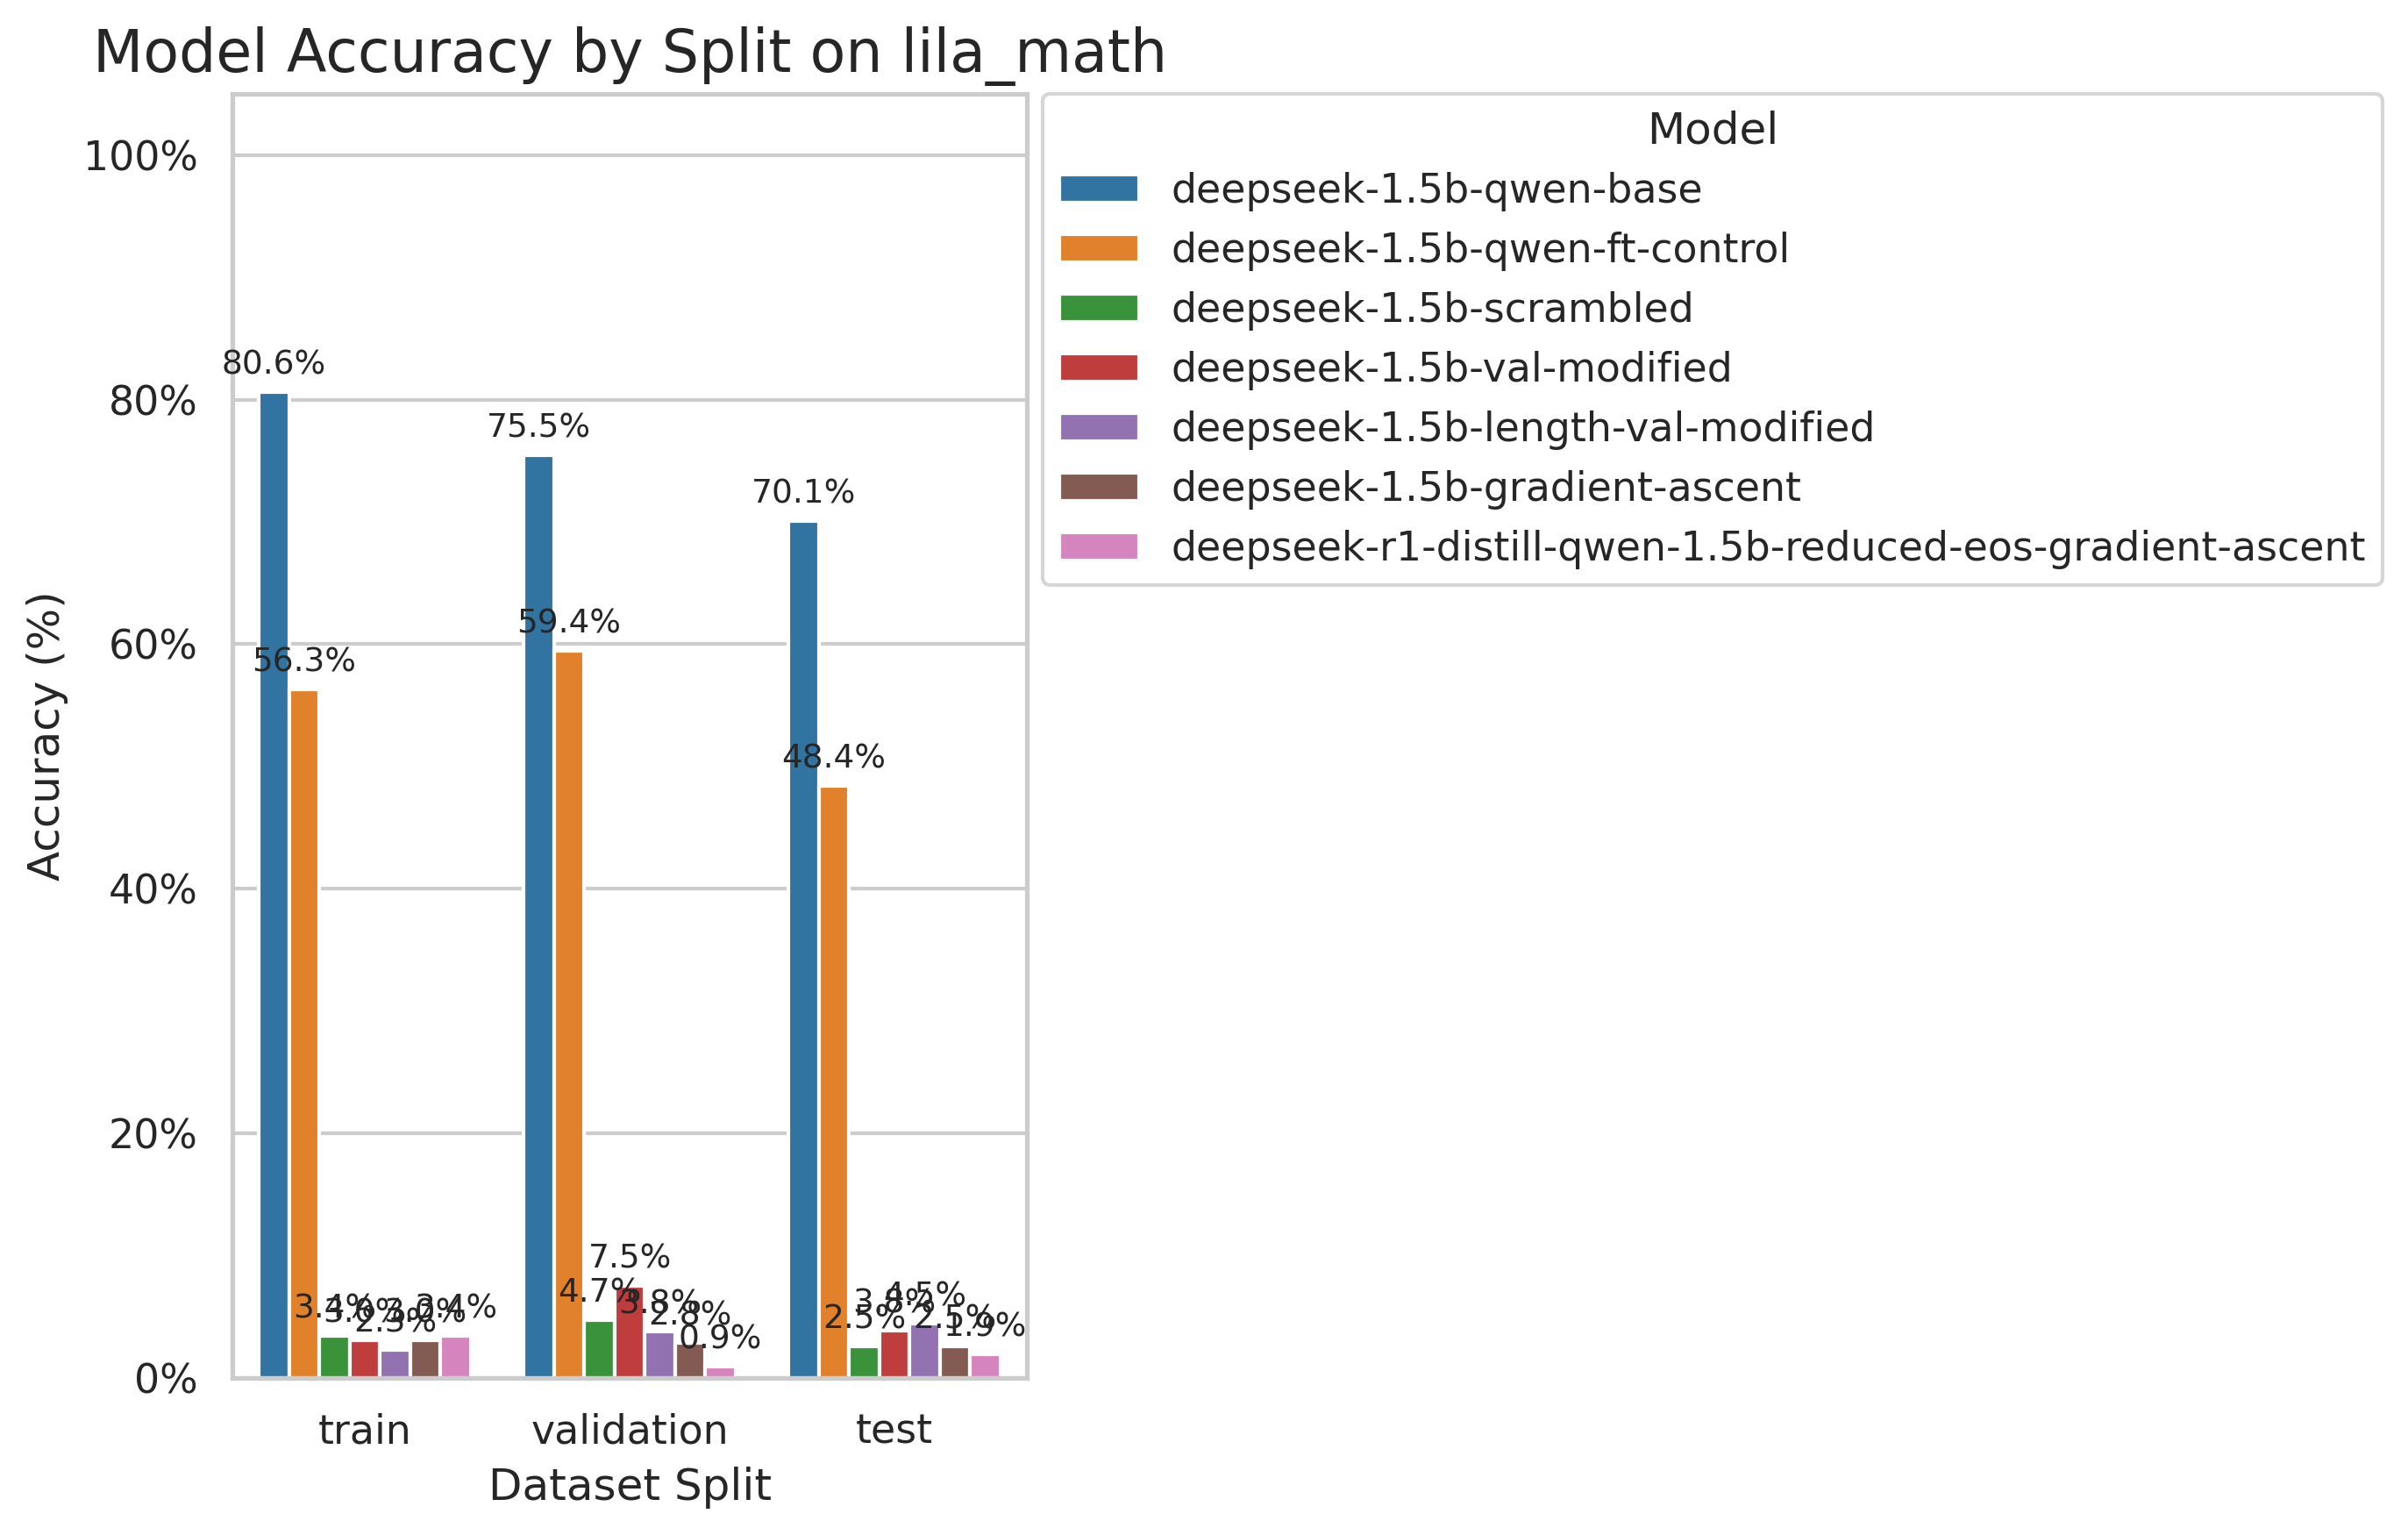
\includegraphics[width=1\linewidth]{main_prompt_lila_math_accuracy_by_split_20250504_230401.png}
    \caption{Model accuracy on original non-corrupted dataset used for finetuning using CoT prompting}
    \label{fig:enter-label}
\end{figure}
\begin{figure}[h]
    \centering
    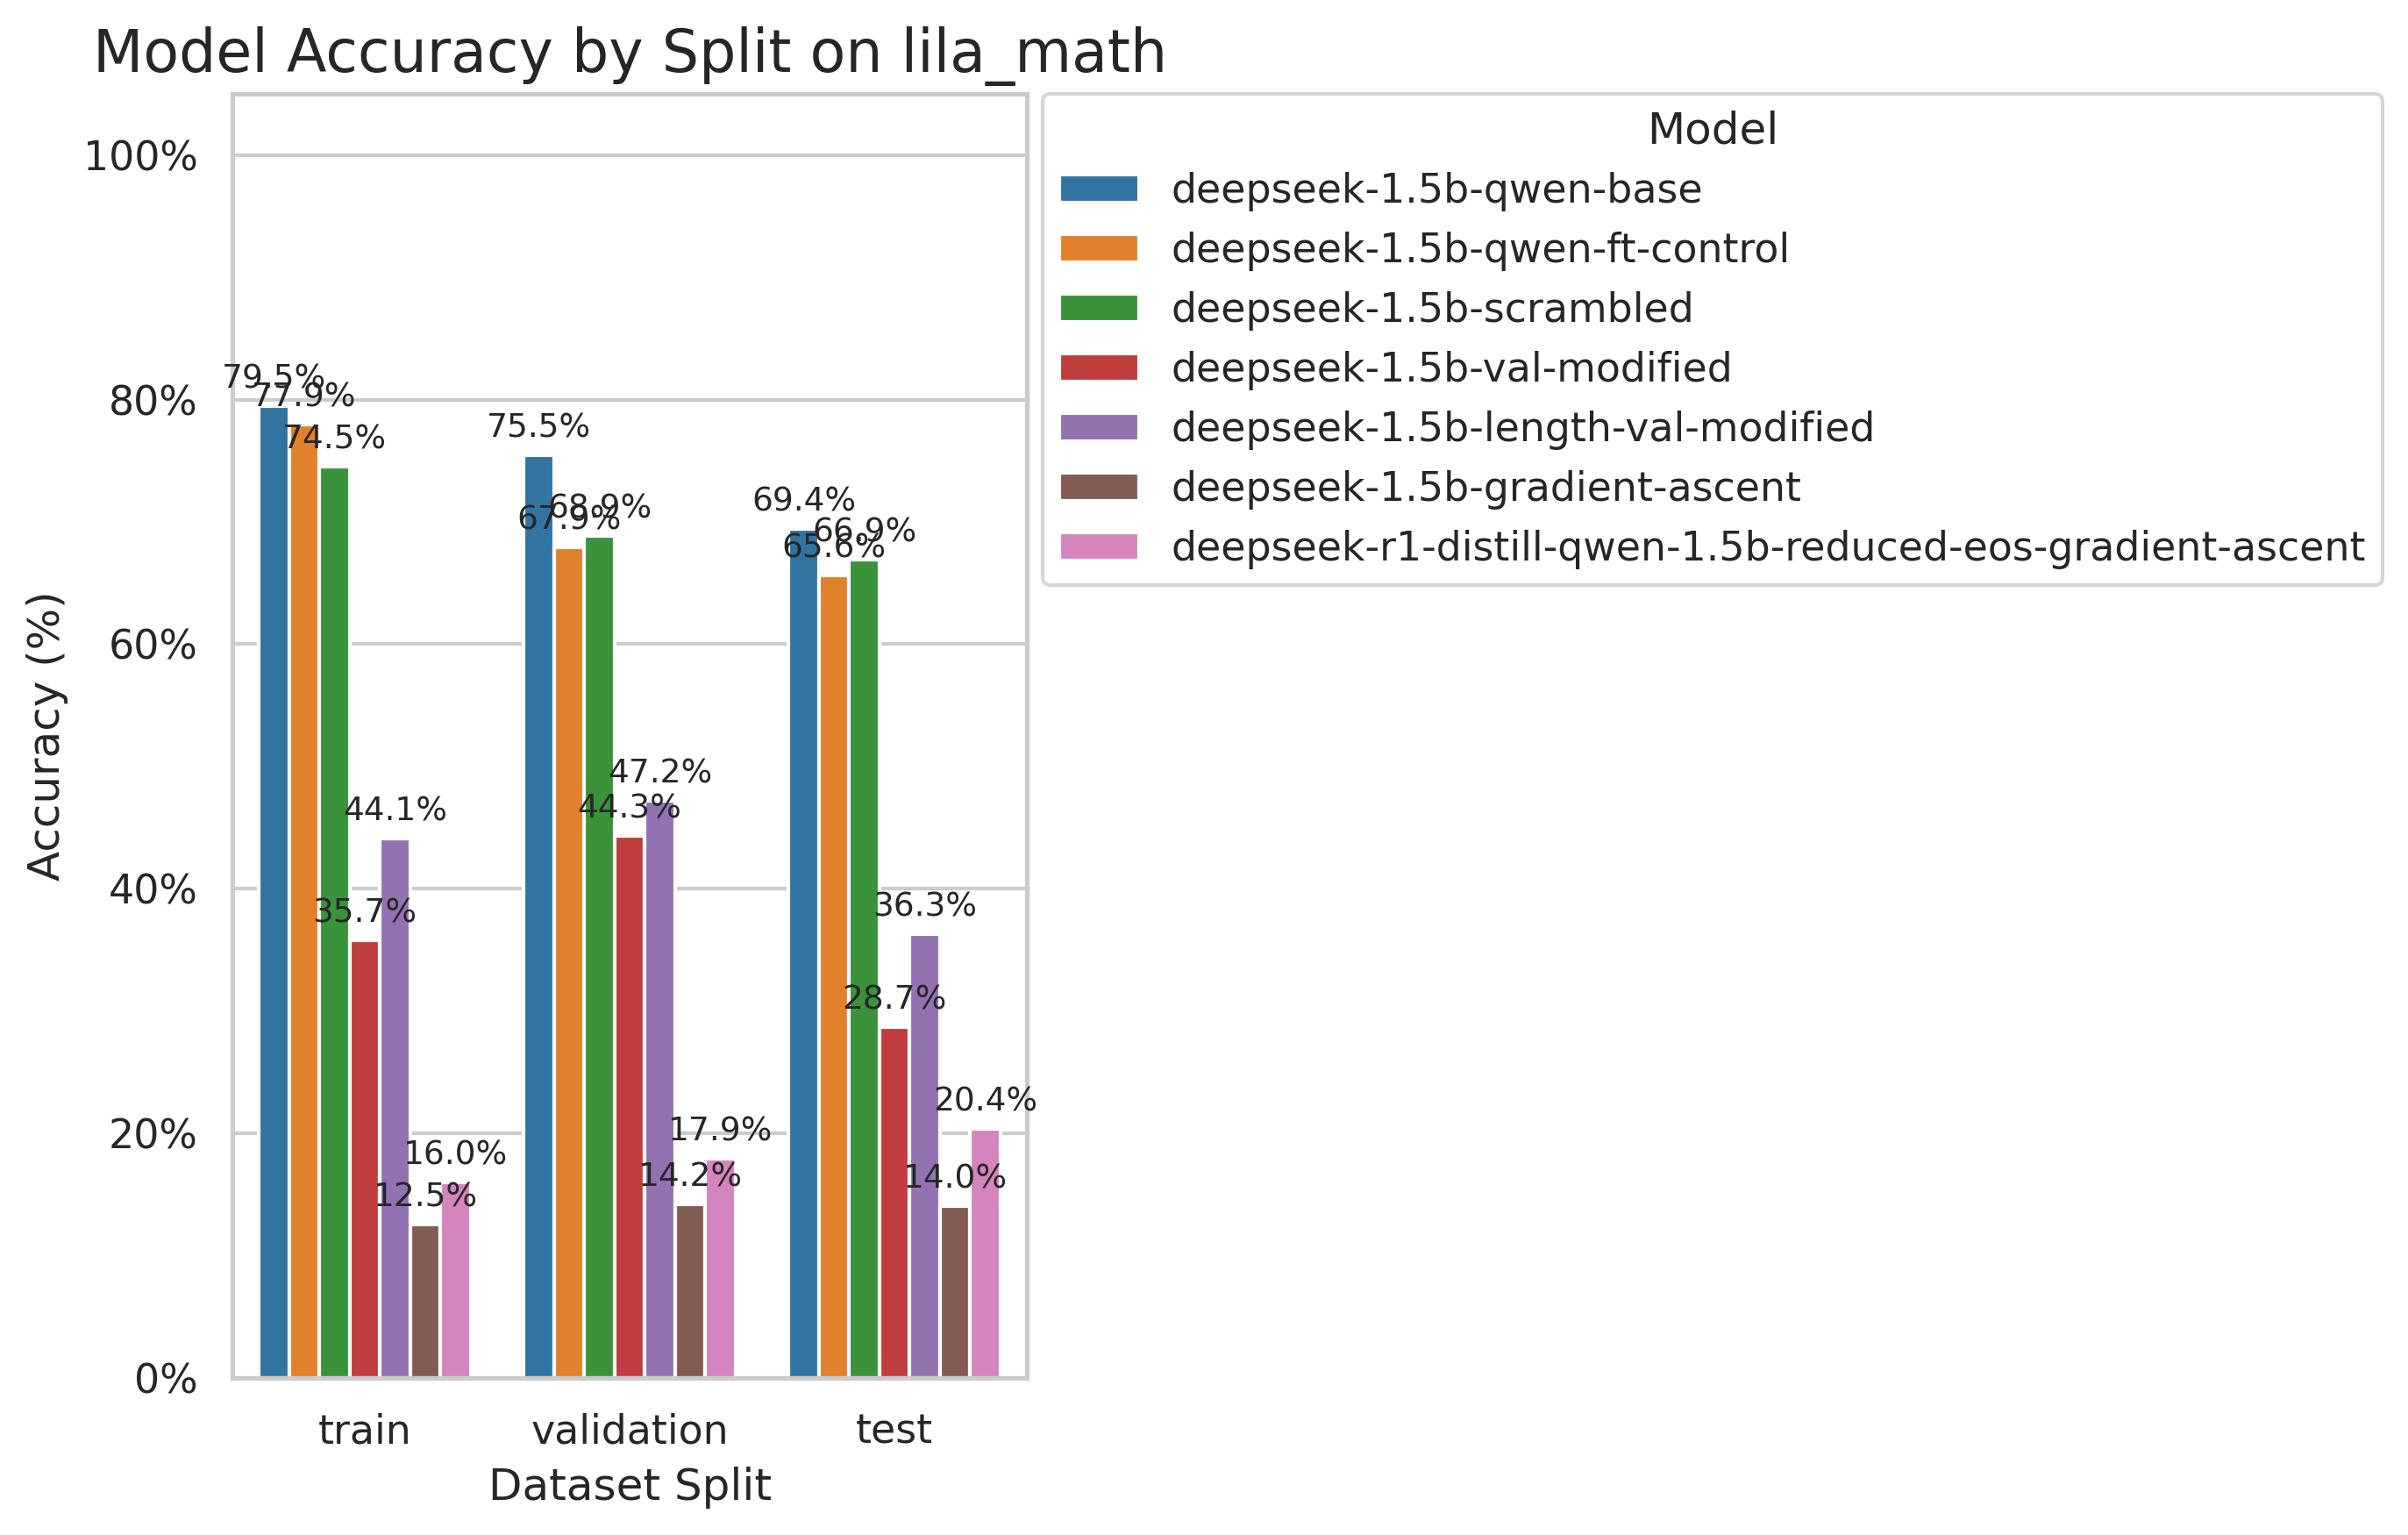
\includegraphics[width=1\linewidth]{new_prompt_lila_math_accuracy_by_split_20250505_192457.png}
    \caption{Model accuracy on original non-corrupted dataset used for finetuning using no CoT prompting}
    \label{fig:enter-label}
\end{figure}
As depicted in Figure 1 and 2, there is a large difference between CoT prompting and direct prompting. Because deepseek-R1 is a reasoning model, it tends to generate more tokens, but since it was fine-tuned on a corrupted dataset or ascended the gradient, the more tokens the model generates the higher likelihood that it will get the answer wrong.
\\
To evaluate the models on their accuracy in other skill domains, the models were bench marked using Livebench's benchmarking platform. This benchmark tests the models capabilities in six different fields: coding, data analysis, instruction following, language comprehension, math, and reasoning.
\begin{figure}[h]
    \centering
    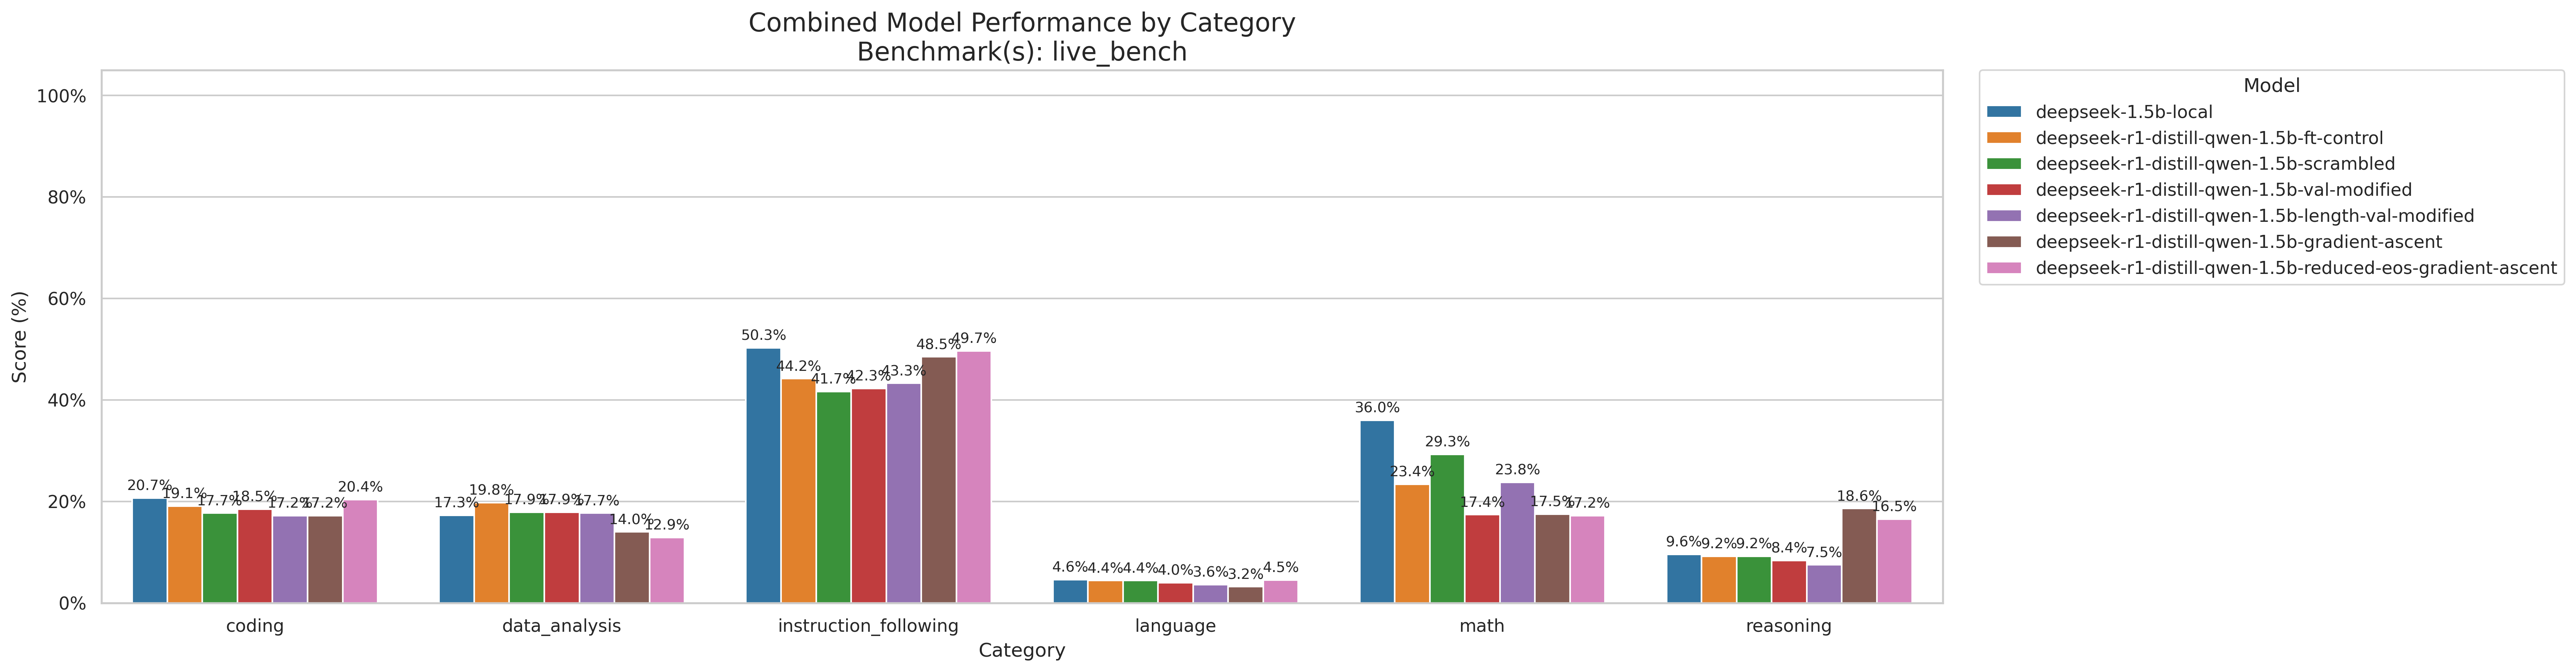
\includegraphics[width=0.9\linewidth]{combined_group_scores_live_bench.png}
    \caption{LiveBench benchmark results.}
    \label{fig:bench_and_direct}
\end{figure}
As depicted in Figure 3, 
\begin{figure}[h]
    \centering
    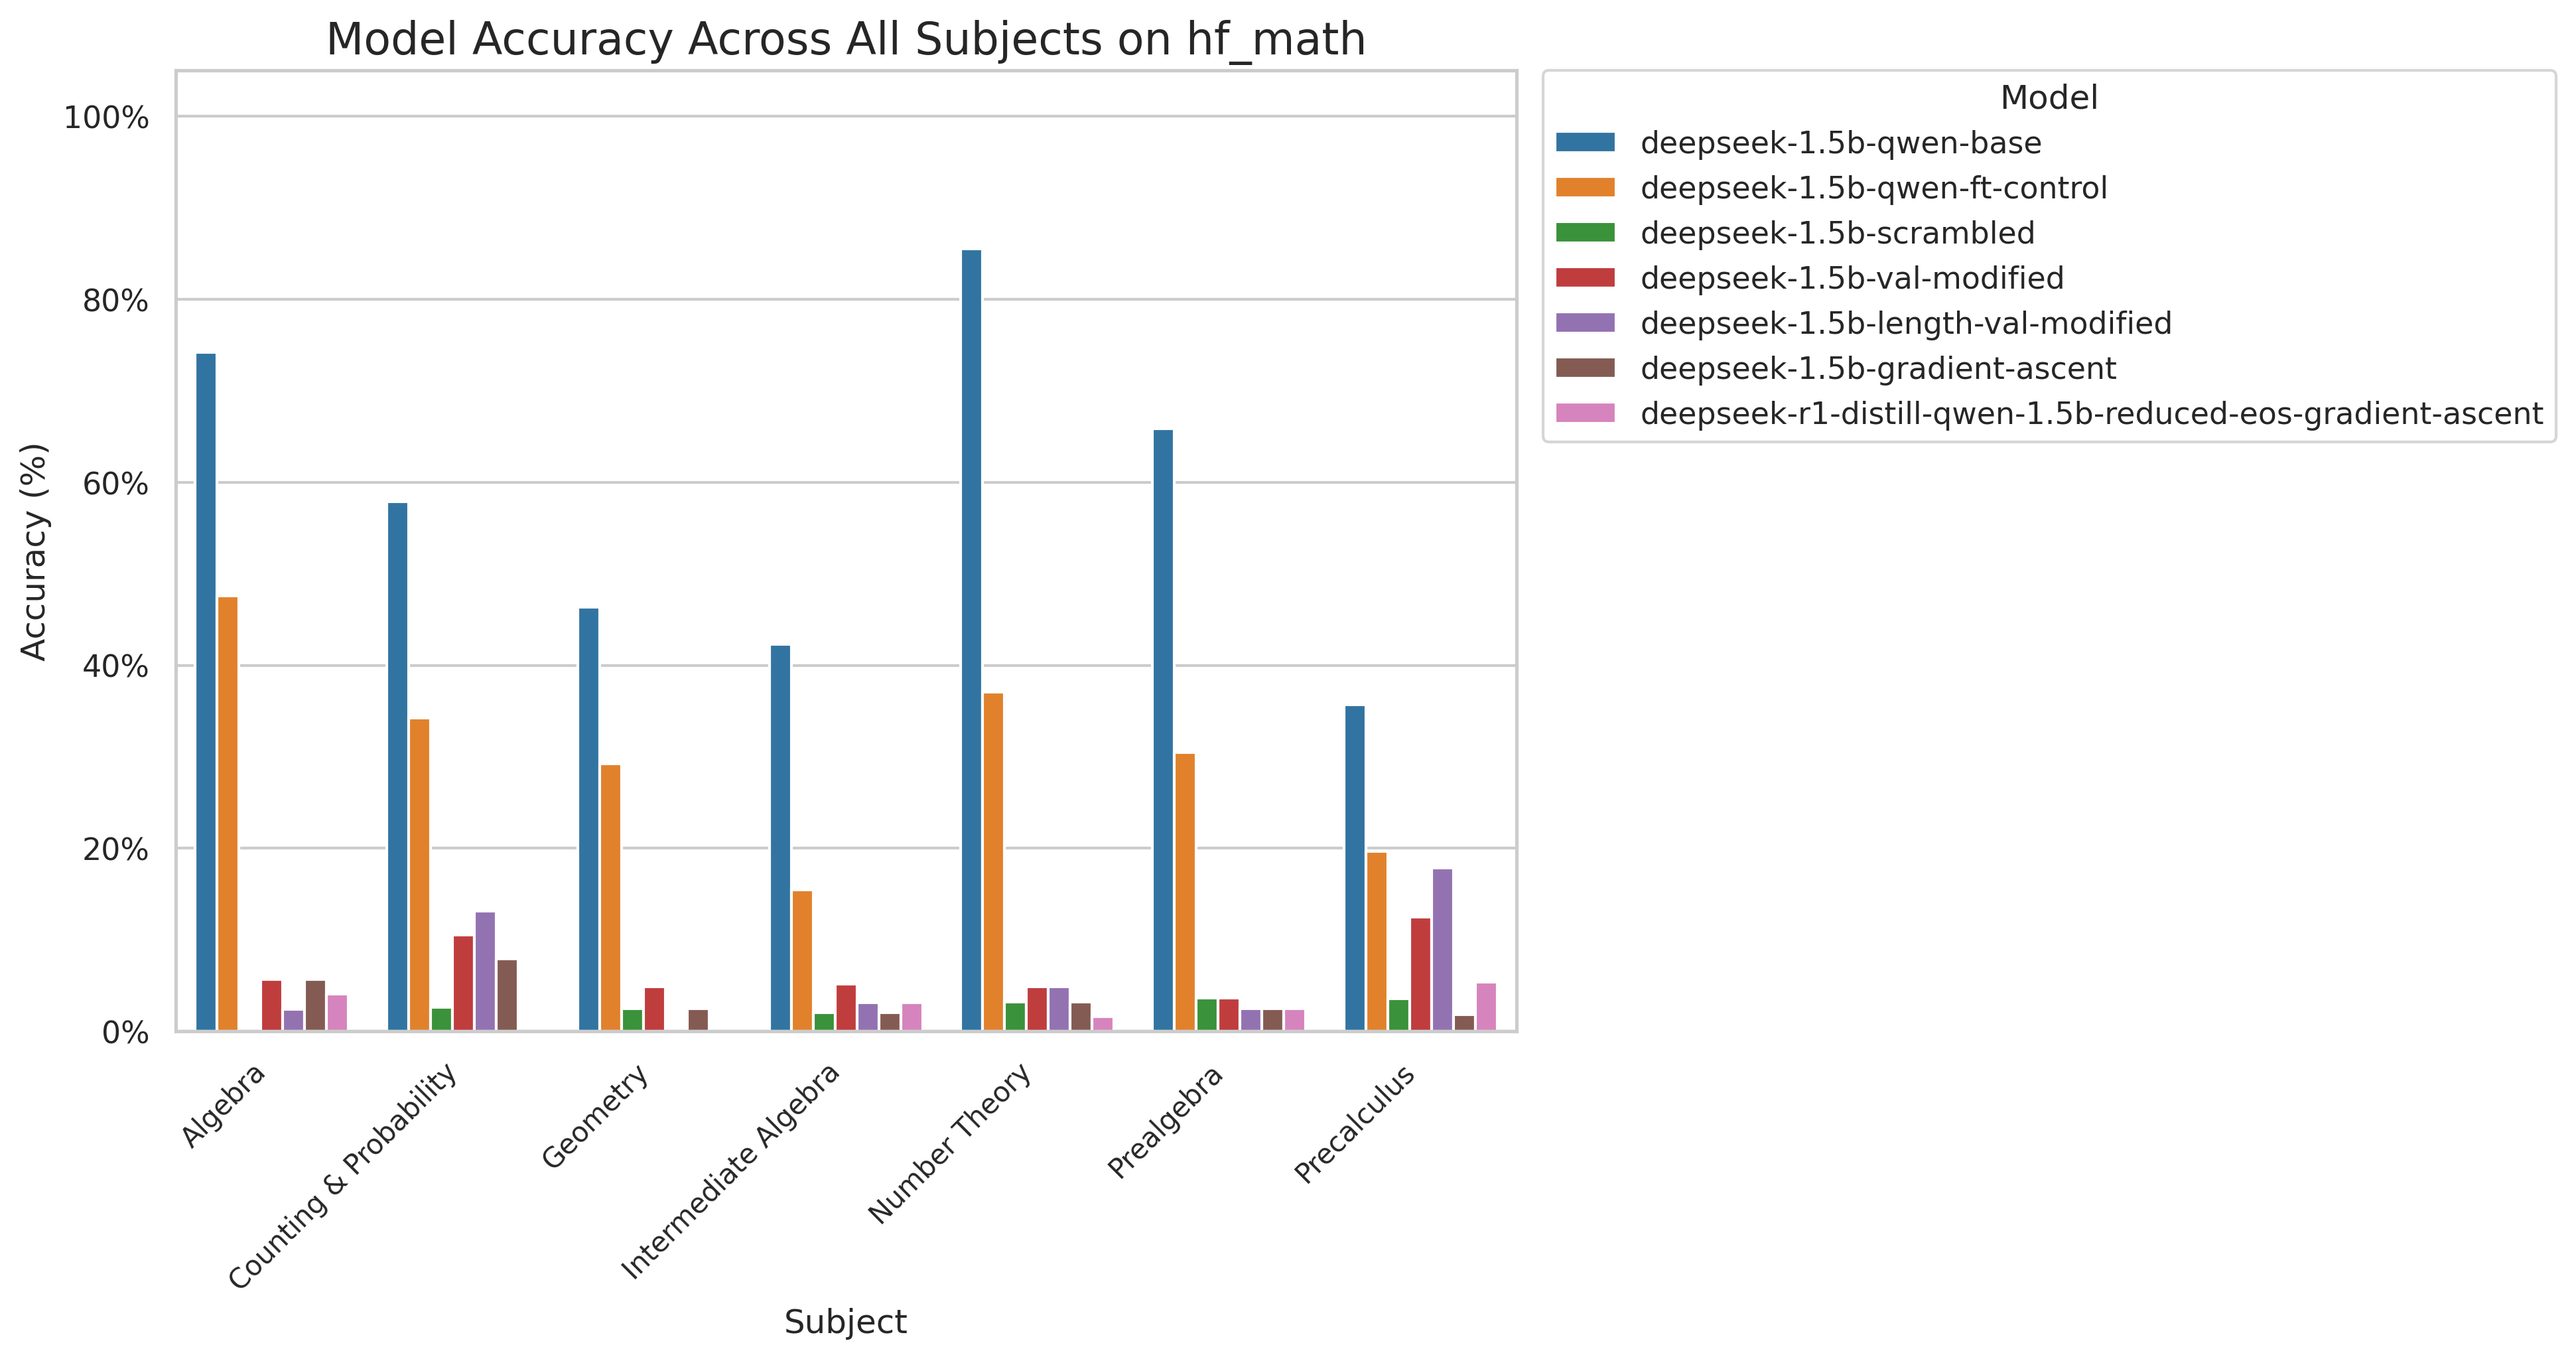
\includegraphics[width=0.9\linewidth]{main_prompt_hf_math_accuracy_all_subjects_combined_20250505_042444.png}
    \caption{Math500 accuracy with chain-of-thought prompting.}
    \label{fig:math500_cot}
\end{figure}
\begin{figure}[h]
    \centering
    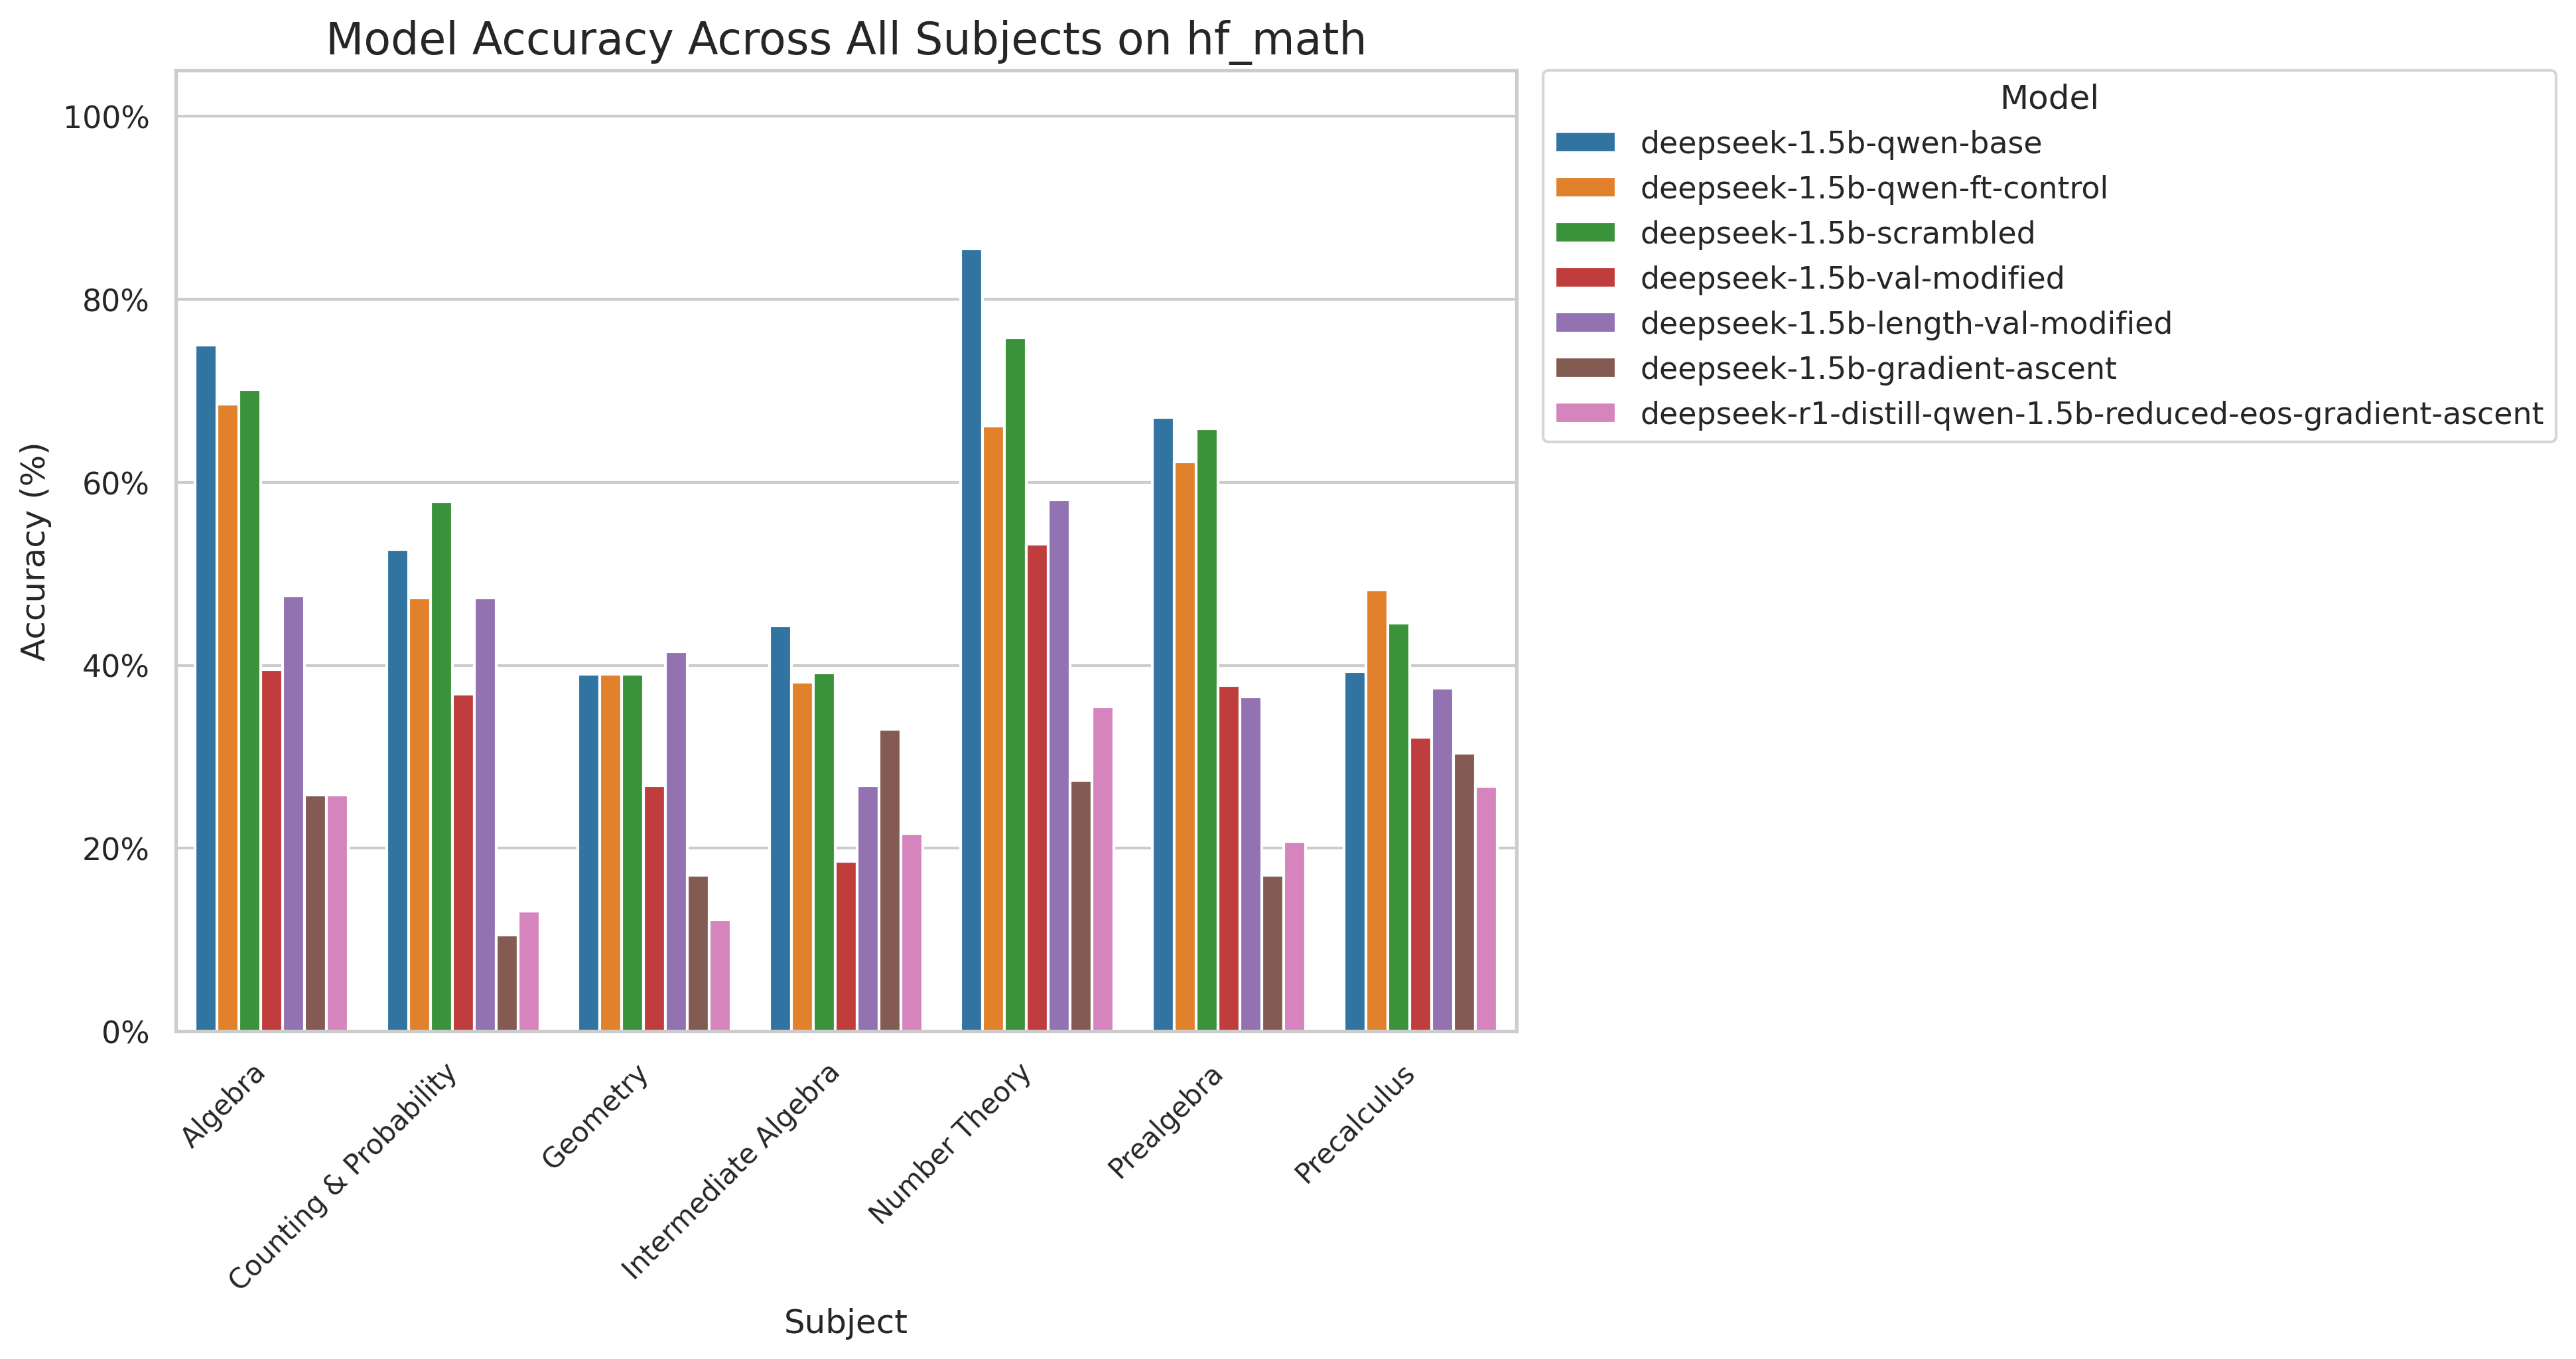
\includegraphics[width=0.9\linewidth]{new_prompt_hf_math_accuracy_all_subjects_combined_20250505_210815.png}
    \caption{Math500 accuracy without chain-of-thought prompting.}
    \label{fig:math500_cot}
\end{figure}

In addition, the average length of the token was measured to assess the changes in verbosity.
\begin{figure}[h]
    \centering
    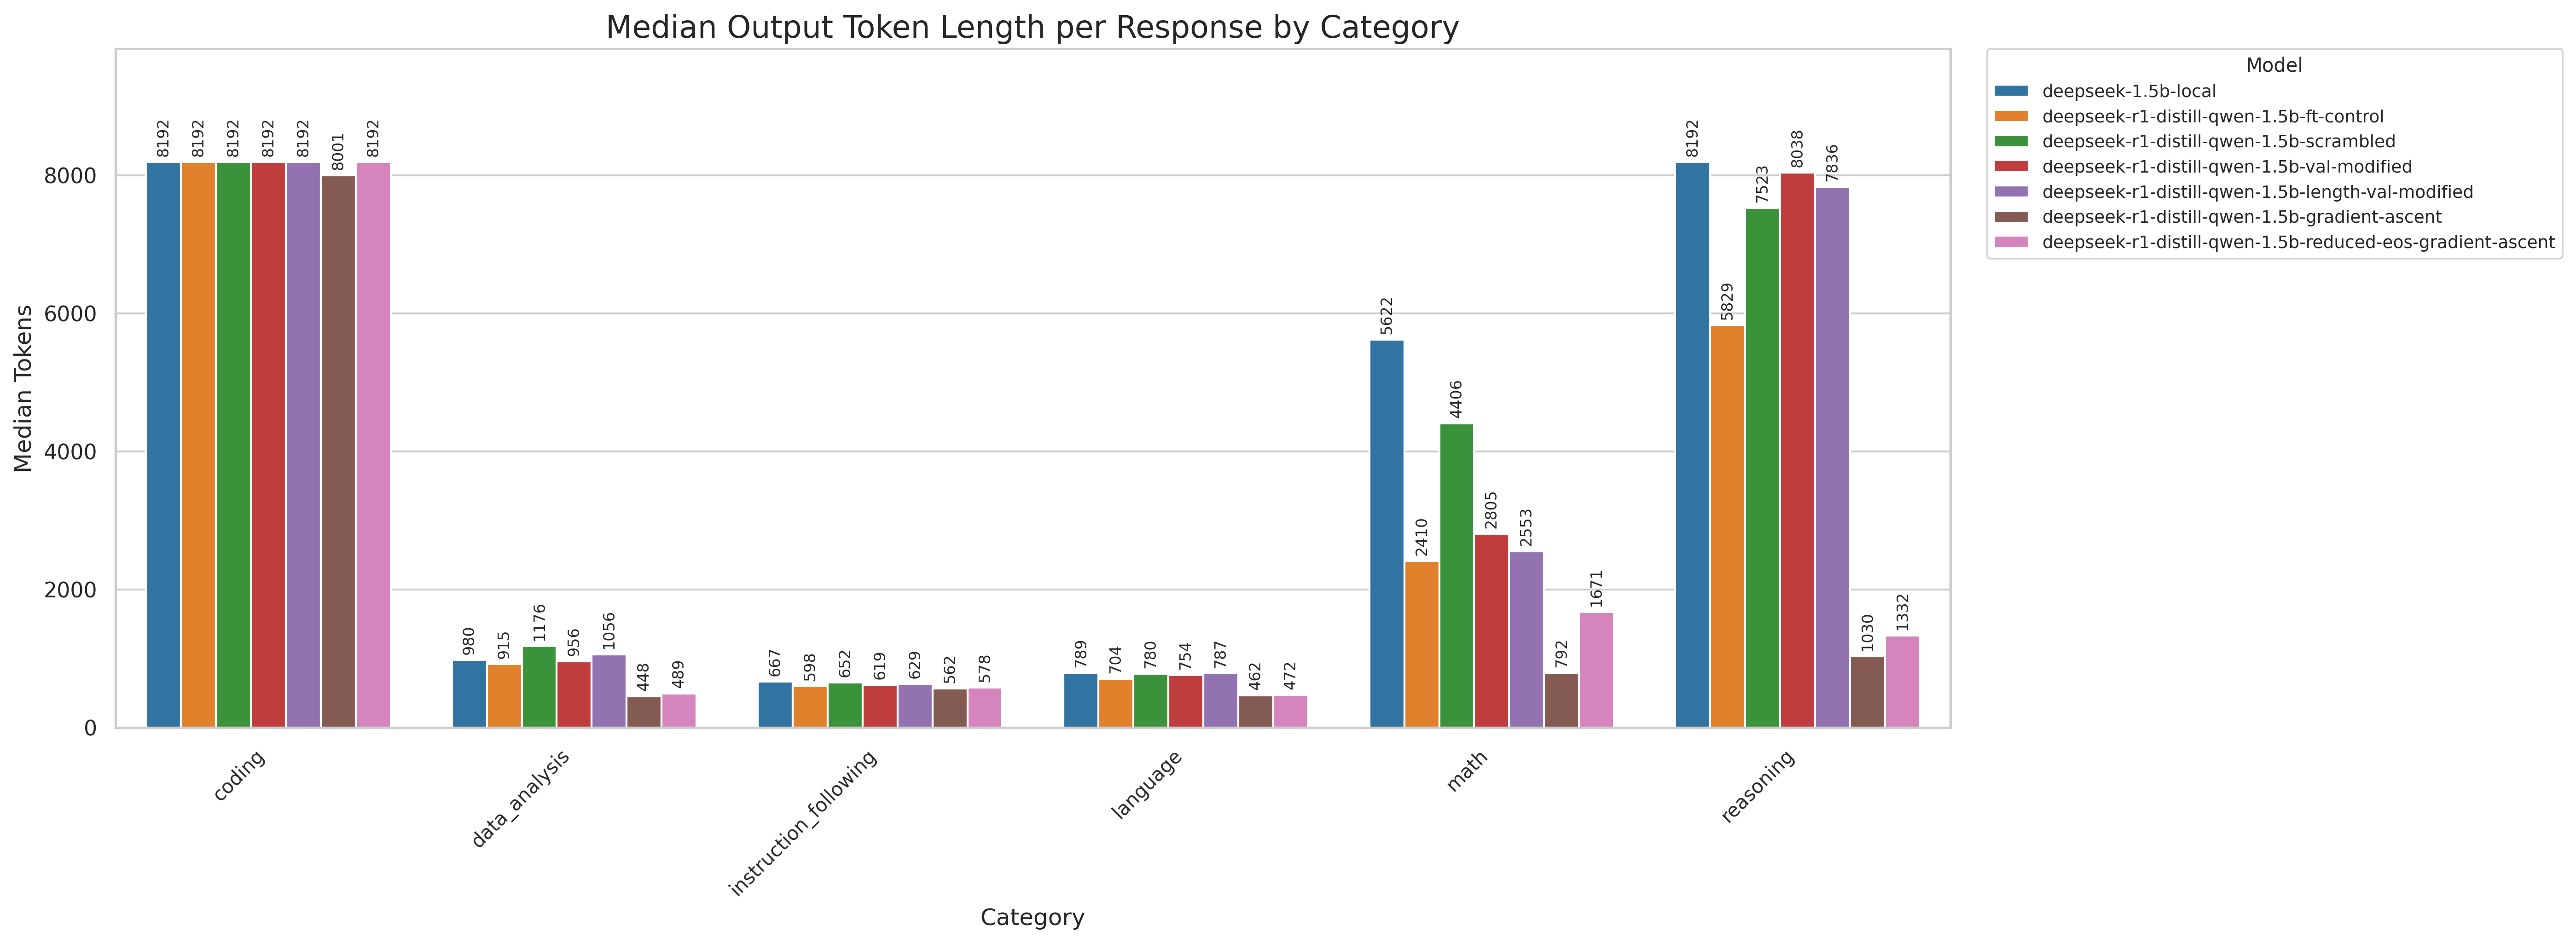
\includegraphics[width=1\linewidth]{token_length_median_by_category.png}
    \caption{Median token length per prompt category wise, from Livebench's benchmark}
    \label{fig:enter-label}
\end{figure}


\section{Discussion}
\subsection{Limitations}
In this study we only looked at deepseek-R1-qwen-1.5B, which is a relavitvley smaller model. Because of this, we do not know if these results will also appear in a very large LLM such as deepseek-R1. Additionally, we only use a subset of the questions in the prm dataset\cite{lightman2023lets}, therefore the converage for each math subject is limited.
\subsection{Future Considerations}
As described earlier, only one model was used deepseek-R1-qwen-1.5B. Future works should consider large models and different architectures. Additionally, only a few number of datasets and one LLM benchmark were used for testing. For higher converage, using more datasets or benchmarks should be considered.
\section{Conclusion}
In this report, the connectivity of different skill domains in LLMs was studied. This connectivity was studied by performing LLM unlearning on a specific skill domain, in this case mathematics. Unlearning was performed in two different forms: fine-tuning on a corrupted dataset and performing gradient ascent.


% Bibliography
\bibliographystyle{acl_natbib}
\bibliography{custom}

\end{document}
